
\chapter{Prototype}
\section{PPi2 Hardware}
\subsection{GPS Module}
    
The \gls{gps} module had to be soldered to the pins. At the beginning we did not want to do that, but without doing that the module did not really connect to the pins so we had to do it.\newline
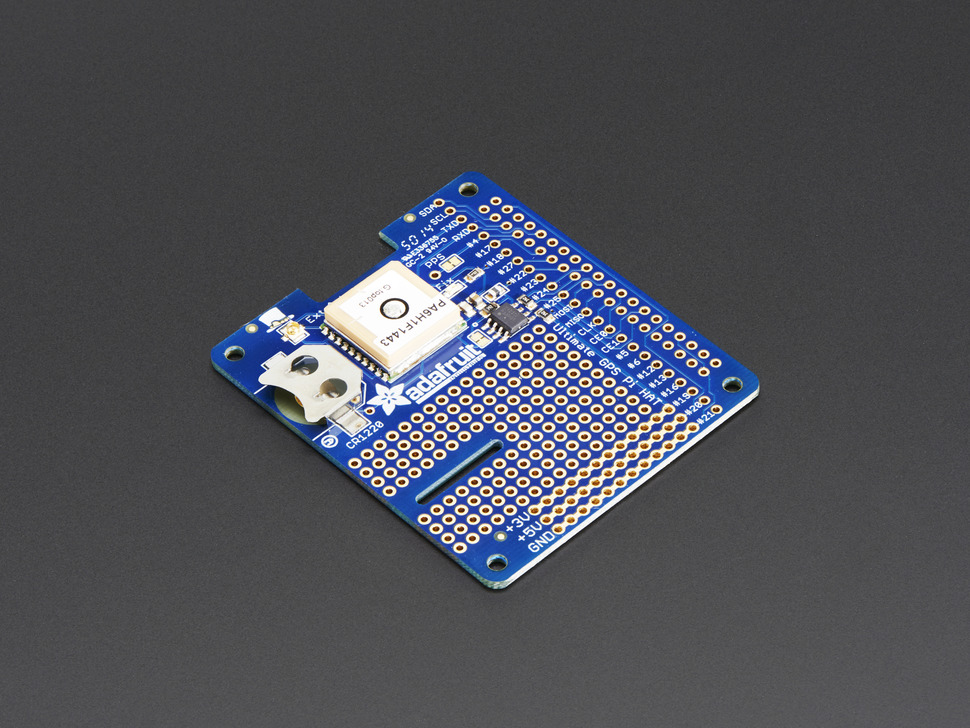
\includegraphics[width=0.48\textwidth]{bilder/GPS}
\subsection{GPS Antenna}
We only used the \gls{gps} antenna for testing. Our problem was that it took really long to get a \gls{gps} signal every time we changed locations. With the antenna it worked much faster. In the final product there will not be a antenna needed. \newline 

\includegraphics[width=0.48\textwidth]{bilder/Antenna}
\subsection{UMTS Stick}
The \gls{umts} Stick is needed for transmitting the data to the \gls{db}.\newline
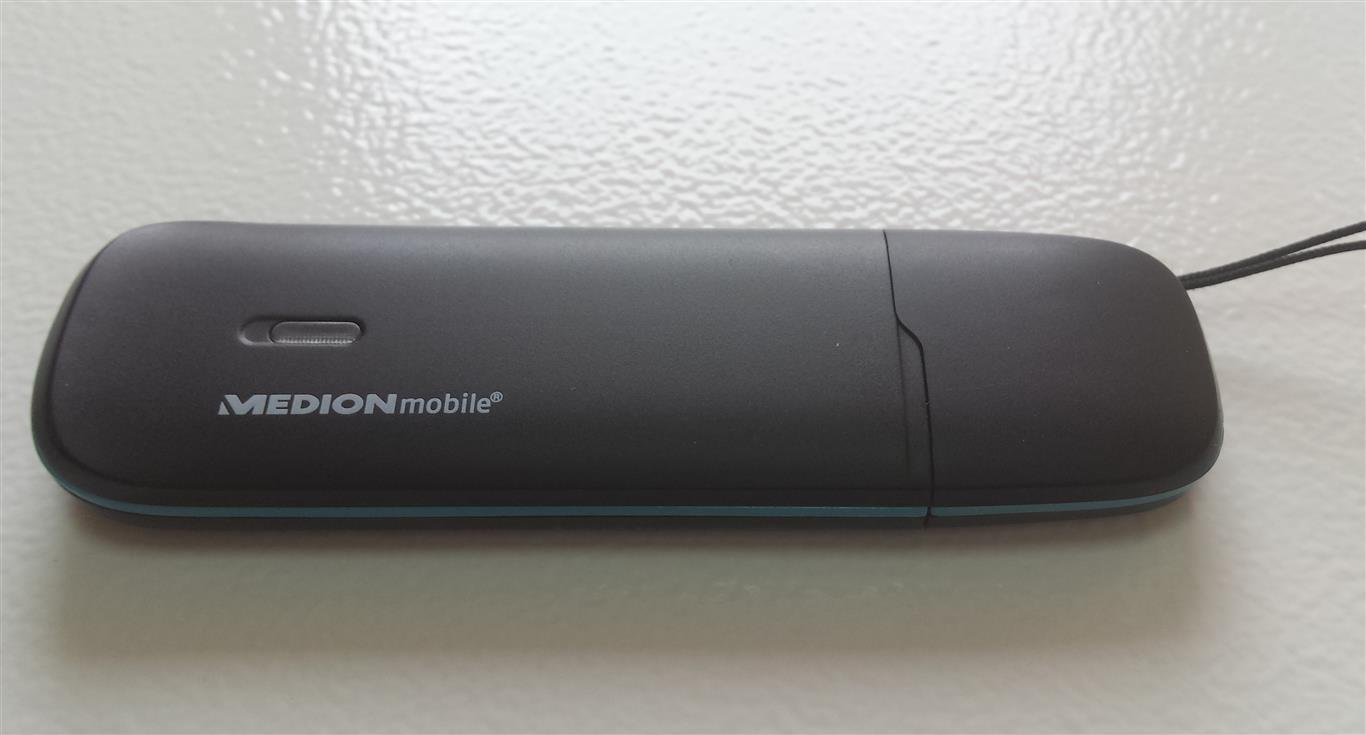
\includegraphics[width=0.48\textwidth]{bilder/Medion_3}
\subsection{UPS}
When the car is switched off the power of the \gls{rpi2} is cut. When the \gls{rpi2} gets power again, it has to do a system check and repair all files. With the \gls{ups} this won’t happen, because the \gls{ups} will shut down the \gls{rpi2}.\newline

\includegraphics[width=0.48\textwidth]{bilder/USV}
\newpage
\subsection{OS}
\subsubsection{Raspbian Wheezy}
When we started our diploma-thesis the most common operation system was and is Raspbian Wheezy. At the beginning we downloaded the image and wrote the .img file on the microSD Card. To start Raspbian Wheezy you always have to connect it to a screen. There you have to configure things like the keyboard layout. You can also do that later with the sudo raspi-config command. After that you have to reboot the \gls{rpi2}.
Since we wanted to have a remote connection, we installed a \gls{tvnc} Server on the \gls{rpi2}. For this we used the the sudo apt-get install tightvncserver. So, to connect to the \gls{rpi2} via a \gls{tvnc} Client we had to start the server with the tightvncserver command. Then the Server started on the Port 5901. To connect to it we had to write the \gls{ip} and the Port 5901 into the \gls{tvnc} Client. And after that we started to configure everything to use the \gls{gps} module.
\paragraph{GPS} \mbox{}\\
First we had to configure, that on the \gls{rpi2} the \gls{uart} pins, which are \gls{gpio} 14 and 15, will communicate with the \gls{rpi2}.\newline
To stop the sending of the debug information, we had to edit the following file /boot/cmdline.txt with the 
\begin{minted}{python}
	sudo nano /boot/cmdline.txt
\end{minted}
command.\newline
There was one line within this text file and there the following text needed to be deleted
\begin{minted}{python}

\end{minted}
console=ttyAMA0,115200 kgdboc=ttyAMA0,115200
 .\newline
So now it looked like this: /dwc\textunderscore otg.lpm\textunderscore enable=0 console=tty1 root=/dev/mmcblk0p2 rootfstype=ext4 elevator=deadline rootwait.\newline
The \gls{rpi2} sends all terminal output over the external serial. To disable this behaviour, we had to edit the the /etc/inittab file. We did this with the 
\begin{minted}{python}

\end{minted}
\textit{sudo nano /etc/inittab} command.\newline
There we had to to comment out one line. The line was:
\begin{minted}{python}
#Spawn a getty on Raspberry Pi serial line
T0:23:respawn:/sbin/getty -L ttyAMA0 115200 vt100
\end{minted}
and after we did that it looked like:
\begin{minted}{python}
#Spawn a getty on Raspberry Pi serial line
#T0:23:respawn:/sbin/getty -L ttyAMA0 115200 vt100
\end{minted}
An interesting thing was, that this file did not exist on the Raspbian Jessie Lite image. There we had to do nothing.\newline
After that we ensured that the Raspbian was up-to-date. At the beginning we did that with the sudo apt-get update, and the 
\begin{minted}{python}
	sudo apt-get dist-upgrade
\end{minted}
command. Then we had to restart the \gls{rpi2}. We waited, but the \gls{rpi2} did not boot. So we connected the \gls{rpi2} to a screen and there it showed us some interesting output like that all CPUs stopped and at the end there was a line that looked like this: \newline
\begin{minted}{python}
	---[ end Kernel panic - not syncing: VFS: Unable to mount root 
	   fs on unknown-block(0,0)
\end{minted}
So we looked what else we could do and found out that we should also use the 
\begin{minted}{python}
	sudo rpi-update
\end{minted}
command before rebooting. So we started all over again, actually we did that many times, because we found other solutions, but they did not help with our problem. \newline
So after we used the 
\begin{minted}{python}
	sudo rpi-update
\end{minted} 
command and rebooted the \gls{rpi2} we could continue.\newline
 Now we had to download and configure the required packages. We had to use the pps-tools and the libcap-dev. We did this with the 
\begin{minted}{python}
	sudo apt-get install pps-tools
\end{minted}
and the sudo apt-get install libcap-dev. After that we also had to install the \gls{gpsd}. We did that with the
\begin{minted}{python}
	sudo apt-get install gpsd gpsd-clients python-gps
\end{minted}
command. The gpsd presents us the data over a small server.\newline
To start the \gls{gpsd} we firstly had to kill all the running \gls{gpsd}s. We did that with the \textit{sudo killall gpsd} commands. After that we could start it, so that we could use with the 
\begin{minted}{python}
	sudo gpsd /dev/ttyAMA0 -F /var/run/gpsd.sock -G
\end{minted}
command.

\paragraph{GPS Data} \mbox{}\\
Since we had to test if the \gls{gps} was working. There are many command line interfaces which present you the data so that you can see something.\newline
There ist the 
\begin{minted}{python}
	sudo cgps -s
\end{minted}
command:\newline
Bild
\newline
then the
\begin{minted}{python}
	sudo xgps
\end{minted}
command:\newline
Bile
\newline
and at last the 
\begin{minted}{python}
	sudo gpsmon
\end{minted}
command:\newline
Bild
\newline
Then we wanted to save the \gls{gps} Data on the \gls{rpi2}. We did this with the 
\begin{minted}{python}
	gpspipe -r | grep '^\$G' | tee test.nmea 
\end{minted}
command.
But since we could not use the \gls{nmea} format, we had to transform it in something like \gls{gpx} or \gls{kml}. Fot that we used the GPSBabel command line program. GPSBabel converts \gls{gps} data into other formats and saves it into a file. But firstly we had to install GPSBabel with the 
\begin{minted}{python}
	sudo apt-get install gpsbabel 
\end{minted}
command. We converted it into both \gls{kml} and \gls{gpx} and for that we had to use these two commands: 

\begin{minted}{python}
	gpsbabel -i nmea -f test.nmea -o kml -F test.kml
\end{minted}
to get a KML file and
\begin{minted}{python}
	gpsbabel -i nmea -f test3.nmea -o gpx -F test3.gpx
\end{minted}
to get a GPX file.
\paragraph{Program} \mbox{}\\
After that we started programming. Since the programming language we all know best is java and it is possible, that our program will also run on smartphone we chose this language. \newline
We looked for an api for java and found one and also a small test program. \newline
But to run a java program we needed java on the \gls{rpi2}. We wanted to use java 8, but there was no real java 8 jdk for the \gls{rpi2}, so we had to use java 7. We did that with the 
\begin{minted}{python}
	sudo apt-get install oracle-java7-jdk
\end{minted}
command.\newline
Everything about the program you can read later.

\paragraph{Auto boot} \mbox{}\\
Although, we started our program mostly from our own notebooks, we wanted it to start automatically after booting. At the end product everything had to start after booting anyway. So we edited the /etc/rc.local file with the \begin{minted}{python}
	sudo nano /etc/rc.local
\end{minted} 
command. At the last position we added the /home/pi/autostart.sh line.\newline
This means, that at the start of the \gls{rpi2} the autostart.sh, which we also created, will be called upon. So now we created the autostart.sh with the 
\begin{minted}{python}
	nano autostart.sh
\end{minted}
command. In in this file we wrote:
\begin{minted}{python}
	#!/bin/sh

	sudo killall gpsd
	sudo gpsd /dev/ttyAMA0 -F /var/run/gpsd.sock -G
\end{minted}
To make the script executable we had to use the \begin{minted}{python}
	chmod +x autostart.sh
\end{minted}
command.

\paragraph{Problems} \mbox{}\\
Here we are going to explain some problems we had and did not mention before.\newline
Since we had a \gls{wlan} stick, we wanted to configure the \gls{rpi2} so that it could connect to a Router. We found out, that we should edit the /etc/network/interfaces file. We did that with the sudo \textit{nano /etc/network/interfaces} command.\newline
At the beginning it looked like this:
\begin{minted}{python}
	auto lo
	iface lo inet loopback

	auto eth0
	allow-hotplug eth0
	iface eth0 inet dhcp

	auto wlan0
	allow-hotplug wlan0
	iface wlan0 inet manual
	wpa-conf /etc/wpa_supplicant/wpa_supplicant.conf

	auto wlan1
	allow-hotplug wlan1
	iface wlan1 inet manual
	wpa-conf /etc/wpa_supplicant/wpa_supplicant.conf
\end{minted}
Then we changed the \gls{wlan} interface.
\begin{minted}{python}
	auto wlan0
	allow-hotplug wlan0
	iface wlan0 inet dhcp
	wpa-ssid "linksys"
	wpa-psk "raspberry"
\end{minted}
This worked, but  if the \gls{rpi2} started and there was no \gls{wlan}, the \gls{rpi2} also did not accept \gls{lan}.
\newpage
\subsubsection{RASPBIAN JESSIE LITE}
Jessie Lite is a command line \gls{os}. Our final product will run on this \gls{os}, because it starts much faster than Raspbian Wheezy. Another thing is, that they stopped updating Raspbian Wheezy since 2015 and since February 2016 you cannot download it on the official side.
\paragraph{Getting started} \mbox{}\\
At the beginning we downloaded the Raspbian Jessie Lite image and wrote the .img file on the microSD Card. \newline
There was the first Problem. \newline
The old Raspbian Wheezy image set the partition size to the maximum while booting. With Jessie Lite we had to do that ourselves. \newline
The next problem was that the ethernet interfaces \gls{ip} was set to manual. Wheezy had set it to auto. So, if we want to have internet access from the beginning, we had to edit the interface file (/etc/network/interfaces) bevor booting the \gls{rpi2}. Since we did it after the boot too, we are going to describe how to do that later and there you can also see what we changed in this file. \newline
The next thing we did, is to edit the boot file(/boot/cmdline.txt). This we had to do so the \gls{gpsd} can get the data from the pins. We did the same as with the ethernet interface later too. With this file, there is no difference when we did it. \newline
In this file we had to remove 
\begin{minted}{python}
	console=ttyAMA0,115200
\end{minted}
in the line. \newline
Then it looked like this: 
\begin{minted}{python}
	dwc\_otg.lpm\_enable=0 console=tty1 root=/dev/mmcblk0p2 
	rootfstype=ext4 elevator=\$ 
\end{minted}
Then we inserted the microSD Card into the \gls{rpi2} and plugged it in.

\paragraph{GPS Configuration} \mbox{}\\
If we had not configured the ethernet interfaces \gls{ip} to manual, we had to connect the \gls{rpi2} to a screen. Then you we edited the interface file(/etc/network/interfaces). This can be done with the 
\begin{minted}{python}
	sudo nano /etc/network/interfaces
\end{minted}
command. \newline
In this file there is a line iface eth0 inet manual and instead of this line we had to write:
\begin{minted}{python}
	auto eth0
	allow-hotplug eth0
	iface eth0 inet auto
\end{minted}
Then we rebooted the \gls{rpi2}, so that we could access it over the \gls{lan}. \newline
Now, if we had not done it before, we edited the boot file(/boot/cmdline.txt) with the command 
\begin{minted}{python}
	sudo nano /boot/cmdline.txt
\end{minted}
There we removed console=ttyAMA0,115200 from the first line.\newline
After that we checked if everything was up to date with the 
\begin{minted}{python}
	sudo apt-get update
\end{minted}
and the 
\begin{minted}{python}
	sudo apt-get dist-upgrade
\end{minted}
command.\newline
Then we had to install different programs, so that the we could get the \gls{gps} data.\newline
First we installed pps tools with the 
\begin{minted}{python}
	sudo apt-get install pps-tools
\end{minted}
command, than the libcap dev with the 
\begin{minted}{python}
	sudo apt-get install libcap-dev
\end{minted}
command and then the \gls{gpsd} with the 
\begin{minted}{python}
	sudo apt-get install gpsd gpsd-clients python-gps
\end{minted}
command.\newline
Since our program is written in java, we also had to install java with the 
\begin{minted}{python}
	sudo apt-get install oracle-java7-jdk
\end{minted}
command.\newline
Some other thing we had to do on the Jessie Lite image, was that we had to edit the \gls{gpsd} file. This file we edited with the 
\begin{minted}{python}
	sudo nano /etc/default/gpsd
\end{minted}
command.\newline
There we had to change many things so below you can see the whole file. 
\begin{minted}{python}
	# Default settings for the gpsd init script and the hotplug wrapper.

	# Start the gpsd daemon automatically at boot time
	START_DAEMON="true"

	# Use USB hotplugging to add new USB devices automatically to the daemon
	USBAUTO="false"

	# Devices gpsd should collect to at boot time.
	# They need to be read/writeable, either by user gpsd or the group dialout.
	DEVICES="/dev/ttyAMA0"

	# Other options you want to pass to gpsd
	GPSD_OPTIONS=""

	# Additionally:
	GPSD_SOCKET="/var/run/gpsd.sock"
\end{minted}

\paragraph{Copy program on RPi2} \mbox{}\\
Now we had to copy the program on the \gls{rpi2}. We wanted to do that via \gls{usb} stick. But there was the next problem. With the old Wheezy image we just connected the \gls{usb} stick. With the Jessie Lite image we had to mount the stick. We created in the /mnt/ directory a new folder named usb(\textit{sudo mkdir usb}). Then we had to mount the \gls{usb} stick. We did that with the
\begin{minted}{python}
	sudo mount /dev/sda1 /mnt/usb/ -o uid=1000
\end{minted}
command. If we wanted to unplug the \gls{usb} stick we had to use the 
\begin{minted}{python}
	sudo umount /mnt/usb
\end{minted}
command.\newline
Then had to copy the .tar.gz file to /opt with the \begin{minted}{python}
	sudo cp gps.tar.gz /opt
\end{minted}
command. To extract it, we use the 
\begin{minted}{python}
	sudo tar xzvf gps.tar.gz
\end{minted}
command.\newline

\paragraph{Autostart(as Daemon)} \mbox{}\\
We created a gps\_rest.service script and put in a folder near our program which we named systemd. Our script looks like this:
\begin{minted}{python}
	[Unit]
	Description=GPS Rest Daemon PaClLaHell
	[Service]
	ExecStart=/sbin/start-stop-daemon --start --quiet --make-pidfile 
	--pidfile /var/run/gps_rest.pid --background --user pi --chuid pi 
	--chdir /opt/gps --exec /usr/bin/java -- -jar GPS_REST.jar
	ExecStop=/sbin/start-stop-daemon --stop --quiet --pidfile 
	/var/run/gps_rest.pid --user pi --chuid pi --exec /usr/bin/java
	Type=forking
	[Install]
	WantedBy=multi-user.target
\end{minted}
Then in /etc/systemd/system/multi-user.target.wants we create a like too the gps\_rest.service (\textit{sudo ln -s /opt/gps/systemd/gps\_rest.service}).
After that we rebooted the \gls{rpi2} and the GPS\_REST.jar started as a Daemon.
To start and stop the Daemon we used these commands:
\begin{minted}{python}
	sudo systemctl start gps_rest.service
	sudo systemctl stop gps_rest.service
\end{minted}
And to get information about the Daemon we used this command:
\begin{minted}{python}
	sudo systemctl status gps_rest.service
\end{minted}

\paragraph{UMTS Stick} \mbox{}\\
Since the \gls{umts} stick is not the newest, it was not that easy to get it to work with the \gls{rpi2}.
\subparagraph{Configure the USB config} \mbox{}\\
At first we had to configure the \gls{rpi2} so that it would accept the stick and accept it as a modem.\newline
We created a file in /opt/gps/udev and there we had to name this file 70-usb-modeswitch.rules. In this fill we had to add this line:
\begin{minted}{python}
	ACTION=="add", SUBSYSTEM=="usb", 
	ATTRS{idVendor}=="0e8d", 
	ATTRS{idProduct}=="0002", 
	RUN+="/usr/sbin/usb_modeswitch -v 0e8d -p 0002 -M 
	'555342431234567800000000000006f0010300000000000000000000000000'"
\end{minted}
Then we had to create a link to the right position, which was /opt/gps/udev/rules/ and we did that with the 
\begin{minted}{python}
	sudo ln -s /opt/gps/udev/rules/70-usb-modeswitch.rules
\end{minted}
command.\newline
After that we could see with the \textit{lsusb} command, that the Id from the stick was right.

\subparagraph{Configuration of the provider}\mbox{}\\
To configurations, we had to change in the super user state, with the 
\begin{minted}{python}
sudo su
\end{minted}
command.\newline
After that we had to create two files with information for ppp. \newline
The first file we had to create in /etc/chatscripts/ and named it hot\_internet.\newline
In this file we had to put these lines:
\begin{minted}{python}
	TIMEOUT 10
	ABORT 'BUSY'
	ABORT 'NO ANSWER'
	ABORT 'ERROR'
	ABORT 'NO CARRIER'
 
	'' 'ATZ'
	'OK' 'ATE1'
	'OK' 'AT+CGDCONT=1,"IP","webaut","0.0.0.0",0,0'
	'OK' 'ATDT*99#'
	'CONNECT' '\c'
\end{minted}
The next file was at /etc/ppp/peers/ and we also named it hot\_internet.\newline
This file looked like this. 
\begin{minted}{python}
	hide-password
	noauth
	connect "/usr/sbin/chat -v -f /etc/chatscripts/hot_internet"
	debug
	/dev/ttyUSB0
	115200
	defaultroute
	replacedefaultroute
	noipdefault
	usepeerdns
	crtscts
	lock
	local
	 
	# Redial and interval
	persist
	holdoff 5
	 
	# No compression
	novj
	novjccomp
	nopcomp
	nodeflate
		 
	# PAP authentication
	 
	# LCP echo messages settings
	lcp-echo-failure 4
	lcp-echo-interval 65535
\end{minted}
After that we could start it with \textit{pon hot\_internet} and stop it with 
\begin{minted}{python}
	poff hot\_internet}
\end{minted}

\subparagraph{Auto boot PPP}\mbox{}\\
When pon/poff worked, we had to configure the /etc/network/interfaces and there we had to add the ppp interface so that the file looked like this:
\begin{minted}{python}
	# interfaces(5) file used by ifup(8) and ifdown(8)
	 
	# Please note that this file is written to be used with dhcpcd
	# For static IP, consult /etc/dhcpcd.conf and 'man dhcpcd.conf'
 
	# Include files from /etc/network/interfaces.d:
	source-directory /etc/network/interfaces.d
	 
	auto lo
	iface lo inet loopback
	 
	auto eth0
	iface eth0 inet dhcp
	 
	allow-hotplug ppp0
	auto ppp0
	iface ppp0 inet ppp
	provider hot_internet
	 
	allow-hotplug wlan0
	iface wlan0 inet manualrp
	    wpa-conf /etc/wpa_supplicant/wpa_supplicant.conf
	 
	allow-hotplug wlan1
	iface wlan1 inet manual
	    wpa-conf /etc/wpa_supplicant/wpa_supplicant.conf
\end{minted}

\newpage
\section{Software Description}
The software of our \gls{rpi2} consists of two threads and a blocking FileObjectQueue. We get the \gls{gps} data from the \gls{api} and upload it via \gls{rest} in the \gls{db}. 
\subsection{Functions}
First of all a logging property file and a gps property file are loaded. The logging property file contains logging information like the saving location and the maximum number of logging files. The gps property file contains the raspberry id, the server \gls{url} and the gps module \gls{ip}.
\subsection{GPS API}
The \gls{api} (Gpsd4java) manages the connection with the \gls{gps} daemon, which covers receiving data, parsing this information into an useful format and supplying it to the “API Thread”. The \gls{gps} data we use consists of the timestamp, coordinateX, coordinateXError, coordinateY, coordinateYError, acceleration, altitude and altitudeError.
\subsection{Tape API}
We implemented this \gls{api}, because of the problem with saving data into an offline file. This \gls{api} provides us a FileObjectQueue where we can put and remove our points and this FileObjectQueue is automatically saved in a file. 
\subsection{Save Thread}
The Save thread reads point data from the FileObjectQueue and sends the data to the \gls{rest} server. When the tracks are written in the database, the Save Thread removes these points from the FileObjectQueue.
\subsection{API Thread}
When the GPS API measures \gls{gps} data, the API Thread gets it from the \gls{api}. The API Thread adds the information about the track and loads it into the FileObjectQueue.
\begin{center}
\includegraphics[width=1\textwidth]{bilder/SoftwareDiagram1}
\end{center} 
\subsection{PHP (REST)}
This part of our software is responsible for the upload into the database. The \gls{rest} server gets the data formatted as \gls{json}.
\begin{center}
\includegraphics[width=1\textwidth]{bilder/SoftwareDiagram2}
\end{center} 
\section{Code Structure}
\subsection{Classes}
\subsubsection{GPS.java}
\paragraph{Constructor}\mbox{}\\
In the GPS.java class, the gpsModuleAddress variable is initialized and gets it is value from the GPSConfiguration.java class.
\paragraph{startGpsdClient}\mbox{}\\
In the startGpsdClient method, the GPS API is initialized and the validate method from the BL.java class is called every time we get data from the GPS API.
\subsubsection{BL.java}
\paragraph{Constructor}\mbox{}\\
In this class the FileObjectQueue is created and initialized by the save.jPoint file and the GsonConverter.java class. 
Then a new track is created and at last the SaveDataThread object is initialized and started.
\paragraph{Validate}\mbox{}\\
Checks if the data from the GPS API is a Number if not it will be set to 0 except the latitude and the longitude. If they are \gls{nan} it will do nothing. 
Then it adds the data from the GPS API to the FileObjectQueue.
\paragraph{ProcessData}\mbox{}\\
This method peeks max 50 and min 15 points from the FileObjectQueue and puts them into a JContainer. Then it sends these points to the DataManager.java class to upload them via the uploadContainer method.
\subsubsection{SaveDataThread.java}
This is an intern Class in the \gls{bl} class which extends Thread.
\paragraph{Run}\mbox{}\\
This override method calls the ProcessData method and then waits 1 second.
\subsubsection{Data Manager.java}
\paragraph{Constructor}\mbox{}\\
Gets the server \gls{url} and puts it on the urlString variable.
\paragraph{UploadContainer}\mbox{}\\
Uploads the JContainer it got, to the Server via \gls{rest} 
\subsubsection{JContainer.java}
This is a beans class that contains attributes, getter and setter methods for the respective attribute and a toString method of the JContainer.
\subsubsection{JPoint.java}
This is a beans class that contains attributes, getter and setter methods for the respective attribute and a toString method of the JPoint.
\subsubsection{GPSConfiguration.java}
At the beginning this class loads the logging properties.
\paragraph{InitConfiguration}\mbox{}\\
Reads the properties for the program from a file and sets these values on the specified variables. If a value is not in the file, it sets a default value. And at the end it closes the file.
\subsubsection{GsonConverter.java}
This class is a converter class that has implemented a FileObjectQueue Converter. In the method from, the bytes from the file are converted, so that they can be saved on the FileObjectQueue. In the toStream method, it is the other way round, so the FileObjectQueue is saved on a file.
\subsection{Class Diagram}
\begin{center}
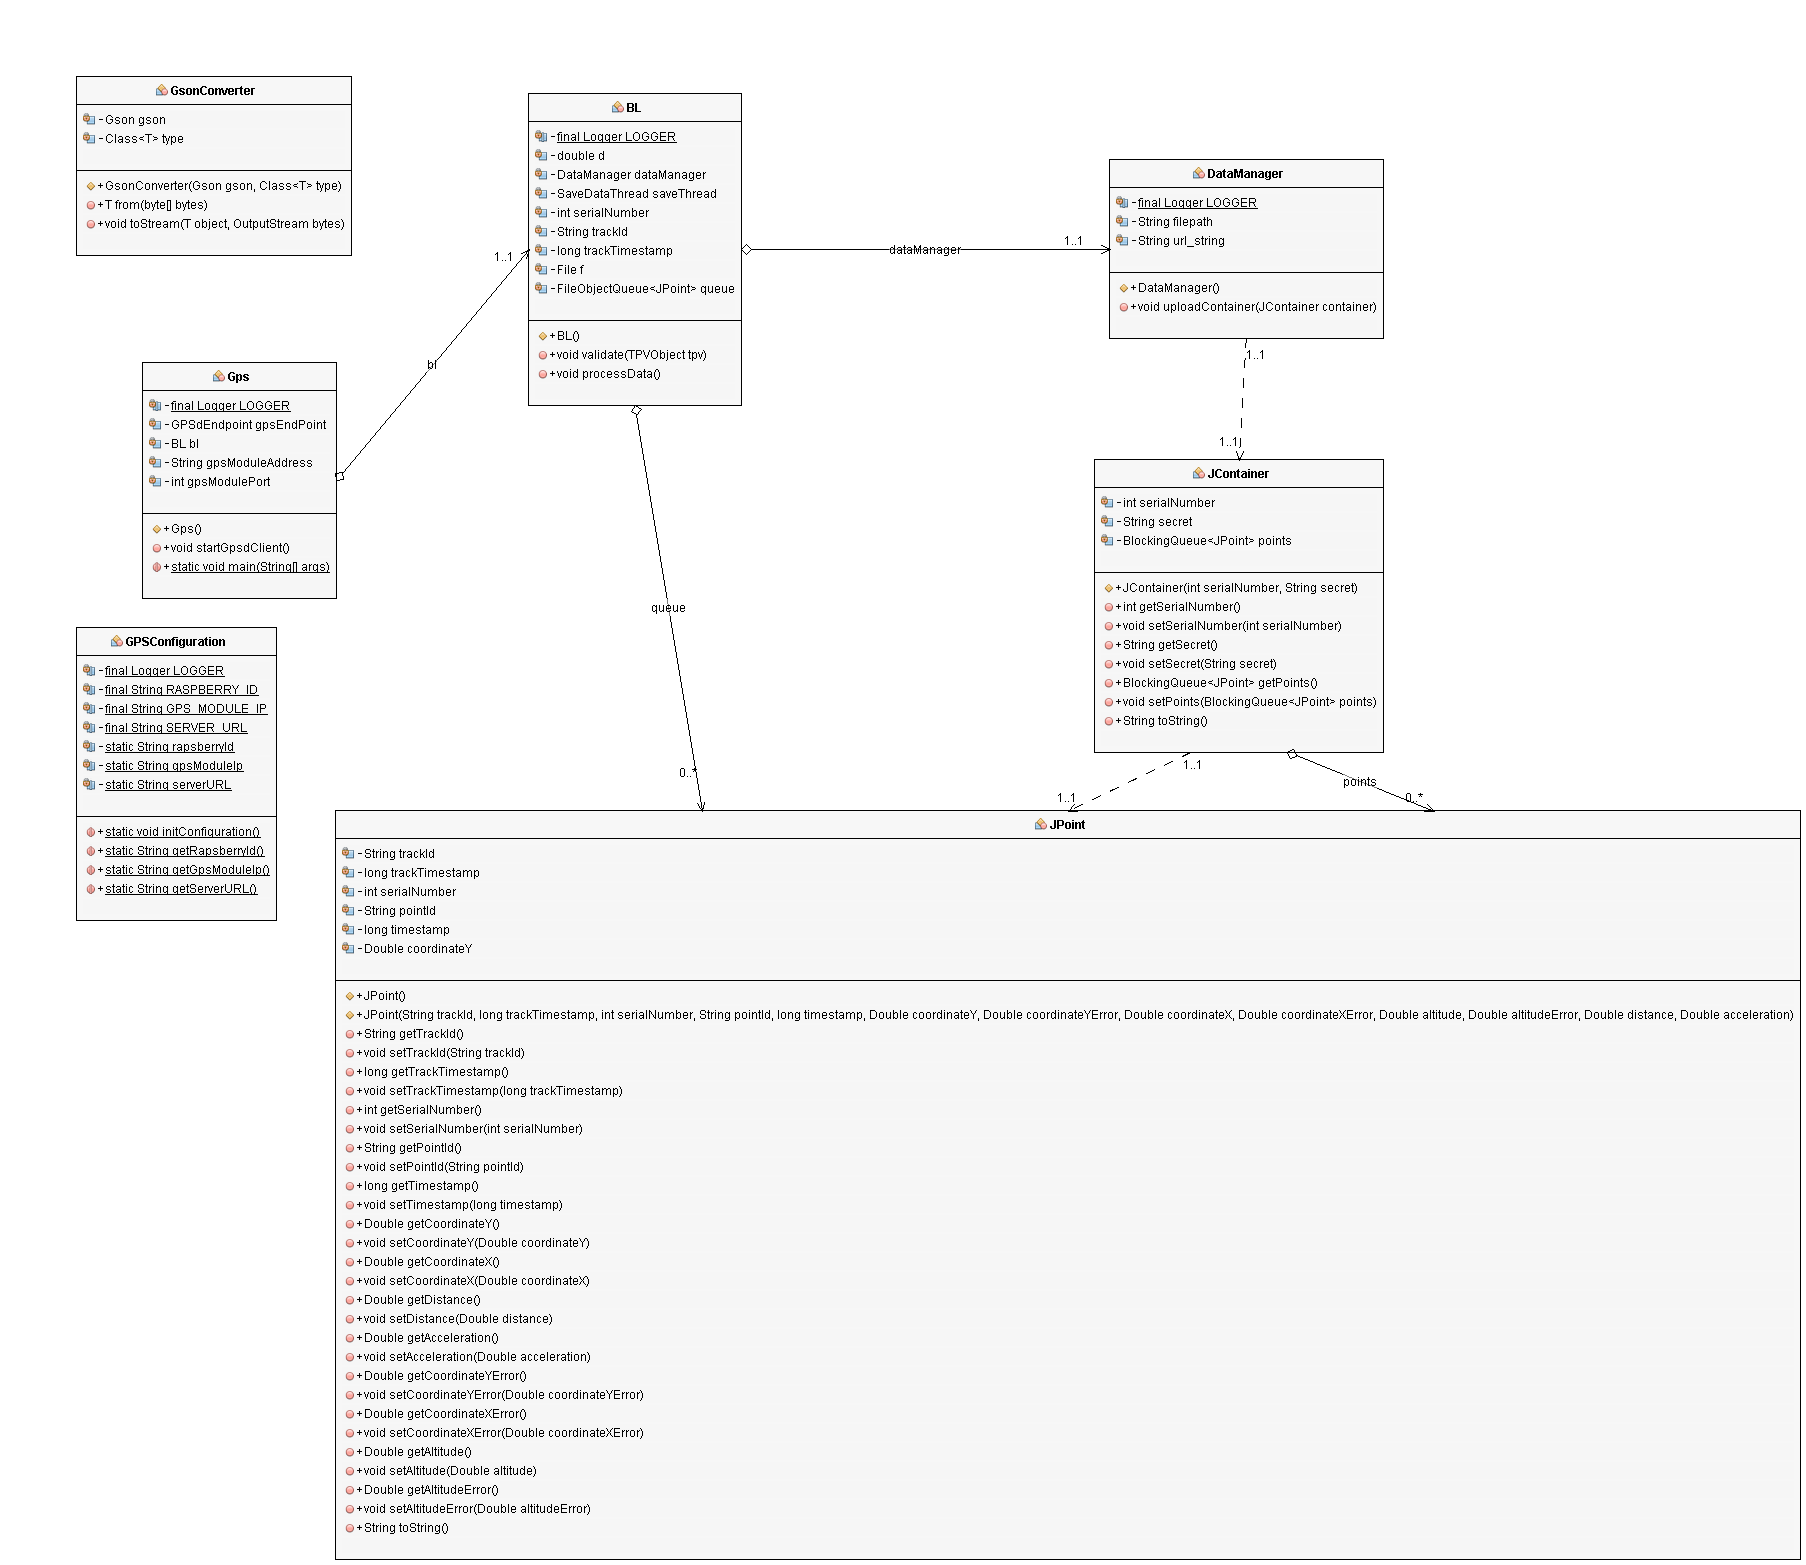
\includegraphics[width=1\textwidth]{bilder/GPS_REST_UML_Diagram}
\end{center}
\section{Problems}
\subsection{Uploading into Database}
When we started with this project, we uploaded tracked data directly into the database over a standard java database connection. During our work on this project, we learned the technology hibernate in school so we reconstructed our program and used hibernate. Later our employer told us, that we should use \gls{rest} to upload data for a higher security level and fewer connections to the database and therefore less overhead. We wrote the \gls{rest} \gls{php} script on our own. 
\subsection{Offline Saving}
When the engine stopped while saving data offline, we had a loss of points, because the whole save file we used was overwritten. So we created a copy of this file, removed the data which was already in the database and deleted the original file. Then we renamed the copy to the original file name. Nevertheless, there was still a problem. On the one hand, it was possible that no data was lost, but on the other hand everything could be lost if the power was cut off between deleting the original file and renaming the copy. This is the reason why we use Tape API now. 
\section{Functional Testing}
To ensure functionality of the hardware prototype and the software, we had to do several tests. They reach from logical problems to practical testing on the road.
\subsection{Database Connection Error}
While developing our software, the error handling when loosing database connection was a very important issue. We had to think about different solutions for different code structure because we changed the database connection type. 
\newline \newline
We decided on the connection type which is called \gls{rest}. When using the connection which relies on a working connection, there had to be a backup plan if exactly this connection is not working anymore.
\newline \newline
In which cases does an connection error occur:
\begin{itemize}
\item internet not working
\item database not working/running
\end{itemize}
We decided on saving points, which cannot be uploaded, into a \gls{json} (save.jPoint). This solution proved to be the most fitting idea we thought of. It perfectly handled the described problems, reliably managed points and the saving mechanism worked phenomenal.
\newline \newline
The same concept is used when the database is offline or not working properly. 

\subsection{Inaccuracy of the GPS Coordinates}
After the first tests, where we tried to get \gls{gps} signal, we noticed the inaccuracy of the signal. This inaccuracy gets influenced by several factors. Therefore we had to find out how precise our \gls{gps} coordinates are and how much of an imprecision (part of the \gls{gps} data we get from our module) there is. 
\newline \newline
We evaluated driven tracks and measured how much distance there is between the actual location and the \gls{gps} coordinates received. This difference was about 5 metres, so no problem at all. 
\newline \newline
Due to the fact that we receive how much of an inaccuracy there is in the \gls{gps} data, our partner company can easily extract this information and compensate it in the visualization process. To do that even better, we also saved the deviation and the altitude.

\begin{center}
%grafiken der gefahrenen strecken --> claudio
%\includegraphics[width=1\textwidth]{}
\end{center}

\subsection{No GPS Signal}
When handling the \gls{gps} inaccuracy, we had to take into account that there could be no signal at all. Therefore we had to decide on a solution when receiving this data and how to handle and save it.
\newline \newline
We tried different solutions, but finally decided on not saving them. It is the most efficient way concerning storage, both offline and online.
\newline \newline
What does not saving data when having no signal mean for us:
\begin{itemize}
\item when there is no \gls{gps} signal, there is often also no internet connection
\item which leads to offline stored “null” points
	\begin{itemize}
	\item not saving these null points is the best solution
	\end{itemize}		
\item data extraction for our partner company when displaying the data on maps will be easier
\end{itemize}